\documentclass[10pt]{report}

\usepackage[headings]{fullpage}
\usepackage{scribe}

% Packages
\usepackage{amsfonts}
\usepackage{amsmath}
\usepackage{amsthm}
%\usepackage[letterpaper,margin=1in]{geometry}
\usepackage{epsfig}
\usepackage{color}
\usepackage{array}
\usepackage{pstricks}
\usepackage{pst-plot}
%\usepackage{pstricks-add}

\theoremstyle{plain}
\newtheorem{lemma}{Lemma}
\newtheorem{claim}[lemma]{Claim}
\newtheorem{theorem}[lemma]{Theorem}
\newtheorem{corollary}[lemma]{Corollary}
\newtheorem{prop}[lemma]{Property}

\theoremstyle{definition}
\newtheorem{define}[lemma]{Definition}
\newtheorem{example}[lemma]{Example}

\newtheorem{problem}{Problem}

\newcommand{\E}{\mathbb{E}}
\newcommand{\R}{\mathbb{R}}
\newcommand{\bP}{\mathbb{P}}
\newcommand{\var}{\mbox{\rm var}}
\newcommand{\pr}{\mbox{\rm Pr}}

\def\X{{\cal X}}
\def\Y{{\cal Y}}
\def\cost{{\mbox{\rm cost}}}

\begin{document}

\course{DSE 210}
\coursetitle{Probability and statistics}
\semester{Winter 2016}
\lecturer{}
\scribe{}
\lecturenumber{6}
\lecturetopic{Generative models 2}

\maketitle

\begin{enumerate}

\item A man has two possible moods: {\tt happy} and {\tt sad}. The prior probabilities of these are:
  $$ \pi(\mbox{\tt happy}) = \frac{3}{4},\ \ \ \pi(\mbox{\tt sad}) = \frac{1}{4} .$$
His wife can usually judge his mood by how talkative he is. After much observation, she has noticed that:
\begin{itemize}
\item When he is happy,
  $$ \pr(\mbox{talks a lot}) = \frac{2}{3}, \ \ \pr(\mbox{talks a little}) = \frac{1}{6}, \ \ \pr(\mbox{completely silent}) = \frac{1}{6}$$
\item When he is sad,
   $$ \pr(\mbox{talks a lot}) = \frac{1}{6}, \ \ \pr(\mbox{talks a little}) = \frac{1}{6}, \ \ \pr(\mbox{completely silent}) = \frac{2}{3}$$
\end{itemize}
\begin{enumerate}
\item Tonight, the man is just talking a little. What is his most likely mood?
\item What is the probability of the prediction in part (a) being incorrect?
\end{enumerate}

\item Suppose $\X = [-1,1]$ and $\Y = \{1,2,3\}$, and that the individual classes have weights
$$ \pi_1 = \frac{1}{3}, \ \  \pi_2 = \frac{1}{6},\ \  \pi_3 = \frac{1}{2}$$
and densities $P_1, P_2, P_3$ as shown below.
\begin{center}

  \vskip.2in
  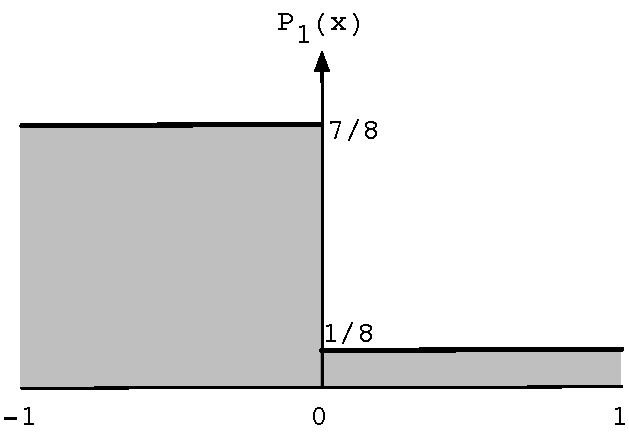
\includegraphics[width=2.5in]{P1.pdf}
  \hskip.5in
  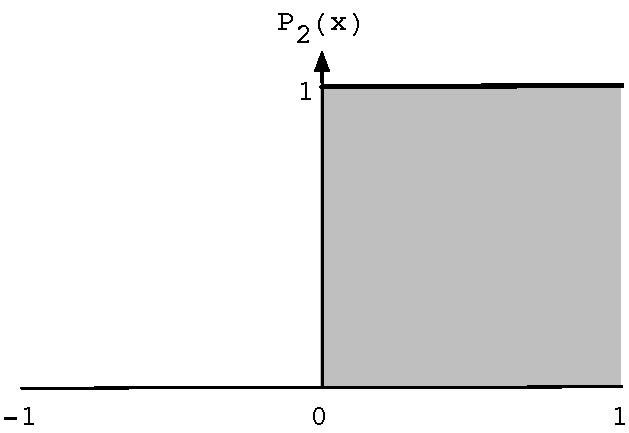
\includegraphics[width=2.5in]{P2.pdf}

  \vskip.2in
  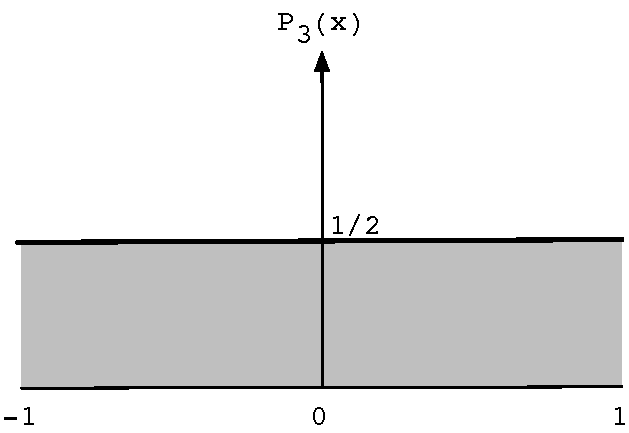
\includegraphics[width=2.5in]{P3.pdf}  
\end{center}

\vspace{.2in}

What is the optimal classifier $h^*$? Specify it exactly, as a function from $\X$ to $\Y$.

\item Would you expect the following pairs of random variables to be uncorrelated, positively correlated, or negatively correlated?
\begin{enumerate}
\item The weight of a new car and its price.
\item The weight of a car and the number of seats in it.
\item The age in years of a second-hand car and its current market value.
\end{enumerate}

\item Consider a population of married couples in which every wife is exactly 0.9 of her husband's age. What is the correlation between husband's age and wife's age?

\item Each of the following scenarios describes a joint distribution $(x,y)$. In each case, give the parameters of the (unique) bivariate Gaussian that satisfies these properties.
\begin{enumerate}
\item $x$ has mean 2 and standard deviation 1, $y$ has mean 2 and standard deviation 0.5, and the correlation between $x$ and $y$ is $-0.5$.
\item $x$ has mean 1 and standard deviation $1$, and $y$ is equal to $x$.
\end{enumerate}

\item Roughly sketch the shapes of the following Gaussians $N(\mu,\Sigma)$. For each, you only need to show a representative contour line which is qualitatively accurate (has approximately the right orientation, for instance).
\begin{enumerate}
\item[(a)] $\mu = \left( \begin{array}{c} 0 \\ 0 \end{array} \right)$ and $\Sigma = \left( \begin{array}{cc} 9 & 0 \\ 0 & 1 \end{array} \right)$
\item[(b)] $\mu = \left( \begin{array}{c} 0 \\ 0 \end{array} \right)$ and $\Sigma = \left( \begin{array}{cc} 1 & -0.75 \\ -0.75 & 1 \end{array} \right)$
\end{enumerate}


\item For each of the two Gaussians in the previous problem, check your answer using Python: draw 100 random samples from that Gaussian and plot it.
  
\item Consider the linear classifier $w \cdot x \geq \theta$, where
$$ w = \left( \begin{array}{c}-3 \\ 4\end{array} \right) \ \ \ \ \mbox{and\ \ \ } \theta = 12 .$$
  Sketch the decision boundary in $\R^2$. Make sure to label precisely where the boundary intersects the coordinate axes, and also indicate which side of the boundary is the positive side.
  
\item {\it Handwritten digit recognition using a Gaussian generative model.} In class, we mentioned the MNIST data set of handwritten digits. You can obtain it from:
  $$ \mbox{\tt http://yann.lecun.com/exdb/mnist/index.html} $$
In this problem, you will build a classifier for this data, by modeling each class as a multivariate (784-dimensional) Gaussian.

\begin{enumerate}
\item[(a)] Upon downloading the data, you should have two training files (one with images, one with labels) and two test files. Unzip them.

In order to load the data into Python you will find the following code helpful:
$$ \mbox{\tt http://cseweb.ucsd.edu/\~{}dasgupta/dse210/loader.py} $$
For instance, to load in the training data, you can use:
$$ \mbox{\tt x,y = loadmnist('train-images-idx3-ubyte', 'train-labels-idx1-ubyte')} $$
This will set $x$ to a $60000 \times 784$ array where each row corresponds to an image, and $y$ to a length-$60000$ array where each entry is a label (0-9). There is also a routine to display images: use {\tt displaychar(x[0])} to show the first data point, for instance.

\item[(b)] Split the training set into two pieces -- a training set of size 50000, and a separate {\it validation set} of size 10000. Also load in the test data.

\item[(c)] Now fit a Gaussian generative model to the training data of $50000$ points:
\begin{itemize}
\item Determine the class probabilities: what fraction $\pi_0$ of the training points are digit 0, for instance? Call these values $\pi_0, \ldots, \pi_9$.
\item Fit a Gaussian to each digit, by finding the mean and the covariance of the corresponding data points. Let the Gaussian for the $j$th digit be $P_j = N(\mu_j, \Sigma_j)$.
\end{itemize}
Using these two pieces of information, you can classify new images $x$ using Bayes' rule: simply pick the digit $j$ for which $\pi_j P_j(x)$ is largest.

\item[(d)] One last step is needed: it is important to smooth the covariance matrices, and the usual way to do this is to add in $c I$, where $c$ is some constant and $I$ is the identity matrix. What value of $c$ is right? Use the validation set to help you choose. That is, choose the value of $c$ for which the resulting classifier makes the fewest mistakes on the validation set. What value of $c$ did you get?
  
\item[(e)] Turn in an iPython notebook that includes:
\begin{itemize}
\item All your code.
\item Error rate on the MNIST test set.
\item Out of the misclassified test digits, pick five at random and display them. For each instance, list the posterior probabilities $\pr(y|x)$ of each of the ten classes.
\end{itemize}
\end{enumerate}

\end{enumerate}

\end{document}
\item A police station wishes to collect statistics on incoming calls. A particular work week is partitioned into $5 \times 8 \times 6 = 240$ intervals of 10 minutes each, and the number of calls received during each interval is noted. Let $N_k$ denote the number of intervals in which $k$ calls were received. The following data was obtained:
\begin{tabular}

\end{tabular}
 
